%!TEX root=main.tex
\subsection{Batch Normalization}
\label{sec:batch_norm}

As discussed in \cite{li2018visualizing} and later in \cite{zhang2018fixup}, the batch normalization (BN) layers are not only important for the neural networks to ensure stable results, but also have significant effects to the loss surface. 
To compare with ResNet-20 which uses batch normalization layers, we adopt the fixup resnet architecture in \cite{zhang2018fixup} which can achieve similar performance without BN layers. 
However, during the training time of fixup resnet, some weights were updated to infinity and corrupted the whole network. 
We are only able to get the first $70$ epochs to compute the loss landscape with final accuracy at roughly $85\%$. 

As shown in \pref{fig:batch-norm-final}, which is more comparable to the 

\begin{figure}[htp]
	\begin{tabular}{cc}
		\subfloat[With Batch Normalization]{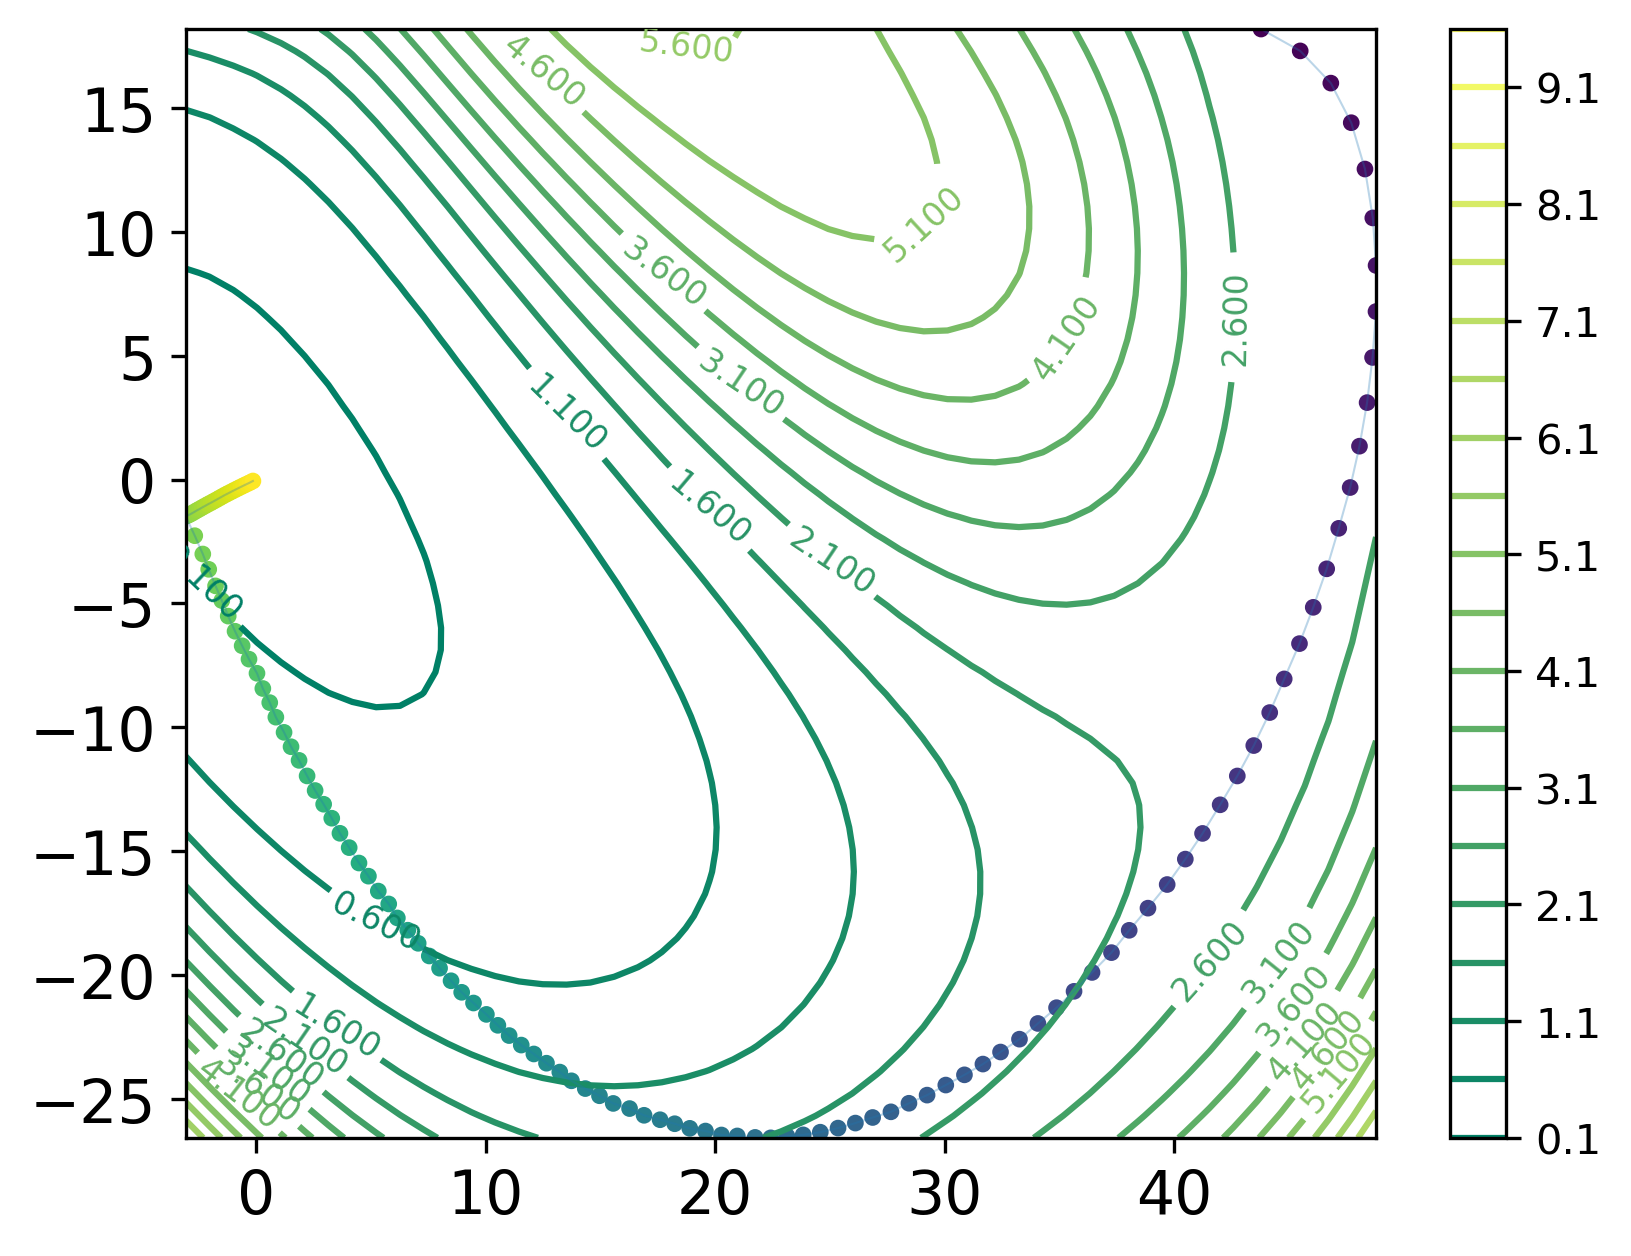
\includegraphics[width =  0.45\linewidth]{results/batch_norm/with_trajectory+contour.png}} &
		\subfloat[Without Batch Normalization]{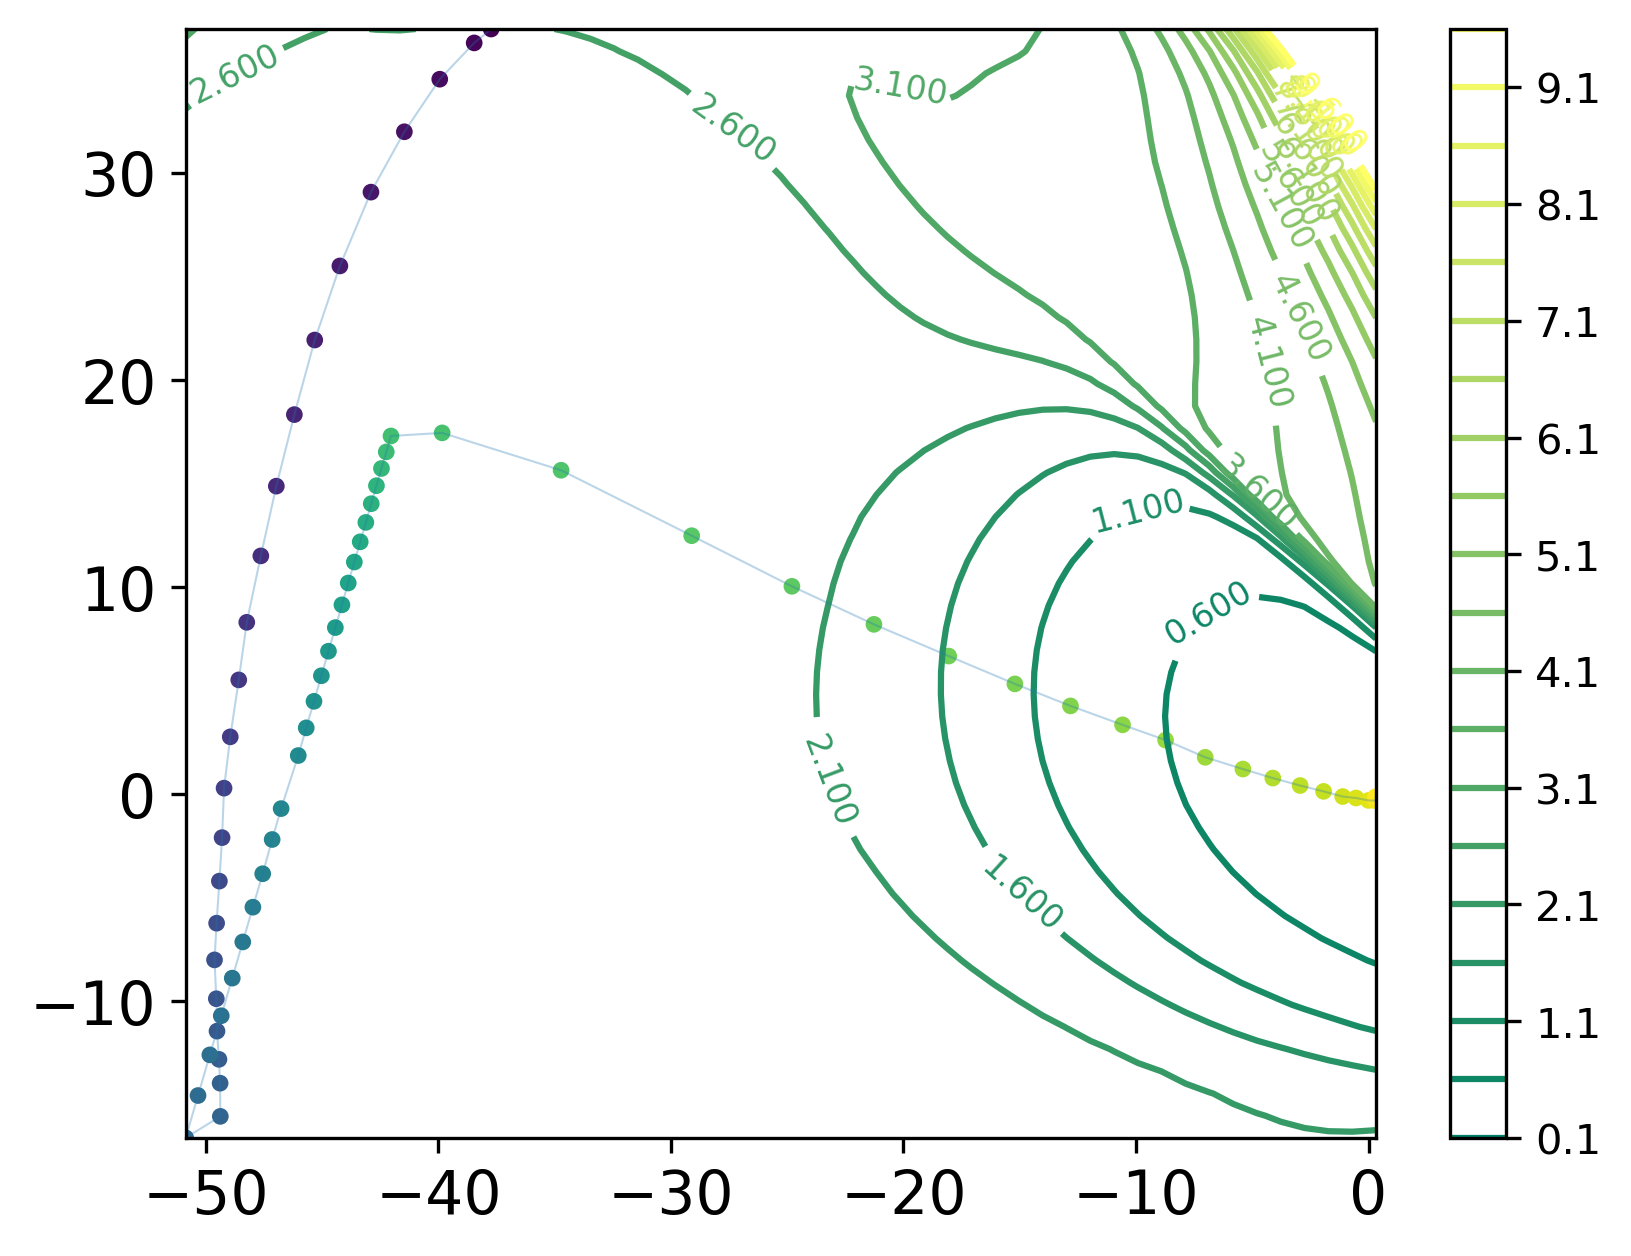
\includegraphics[width =  0.45\linewidth]{results/batch_norm/without_trajectory+contour.png}} 
	\end{tabular}
	\caption{Loss landscapes with/without Batch Normalization}
	\label{fig:batch-norm-final}
\end{figure}

